\documentclass[11pt]{article}
\usepackage[margin=1in]{geometry}
\usepackage{graphicx}
\usepackage{booktabs}
\usepackage{caption}
\graphicspath{{../figures/}}
\begin{document}

\section*{Supplementary material for\\
PhysINR-Zero: zero-shot underwater image enhancement with
physics-constrained coordinate fields, evaluated under a
leakage-guarded re-benchmarking protocol}

This document contains figures that visualise data reported in full in the
main text's tables: the meta-training convergence curve, the LSUI and EUVP
score distributions, and the per-set radar charts. They are referenced from
the main text as Figs.~S1--S4. All plots are vector PDF; raster TIFF
siblings ship in the source package.

\begin{figure}[htbp]
\centering
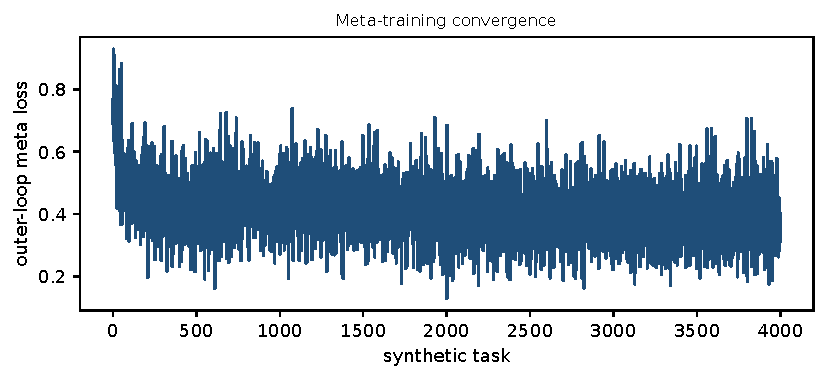
\includegraphics[width=\textwidth]{meta_train_curve.pdf}
\caption*{\textbf{S1} Meta-training curve: outer loss over the 4,000-task run (held-out synthetic tasks).}
\end{figure}

\begin{figure}[htbp]
\centering
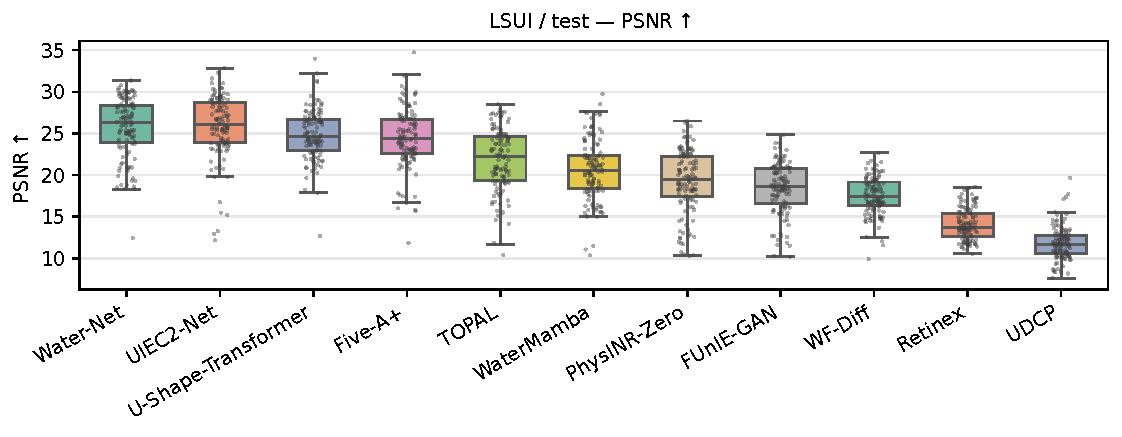
\includegraphics[width=0.48\textwidth]{box_LSUI_psnr.pdf}
\hfill
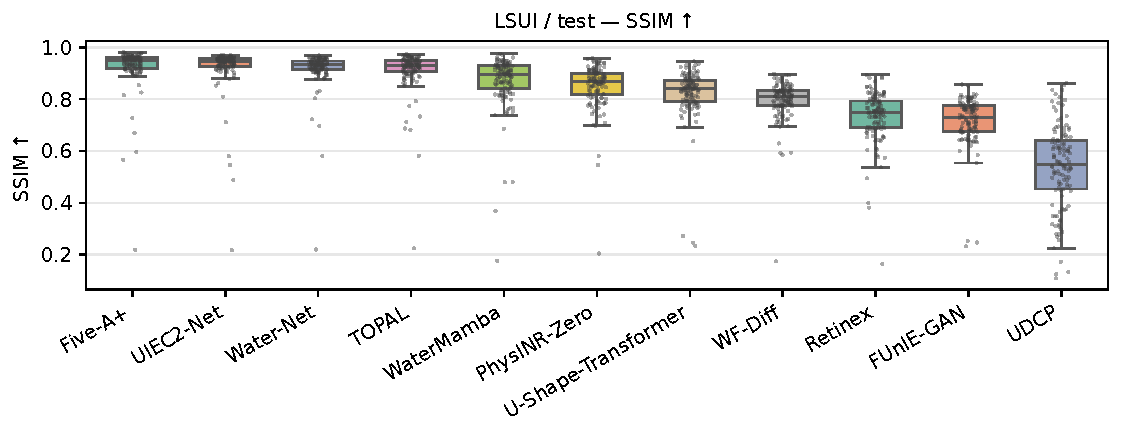
\includegraphics[width=0.48\textwidth]{box_LSUI_ssim.pdf}
\hfill
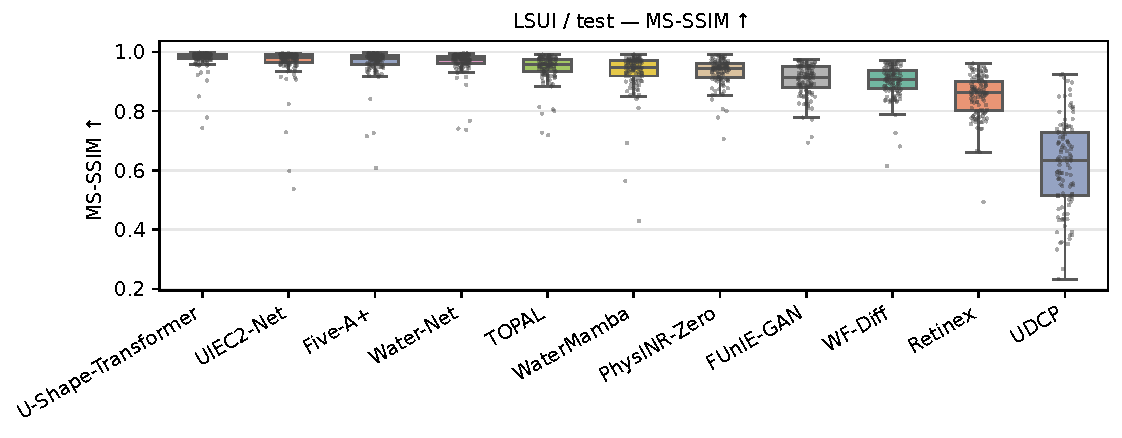
\includegraphics[width=0.48\textwidth]{box_LSUI_ms_ssim.pdf}
\hfill
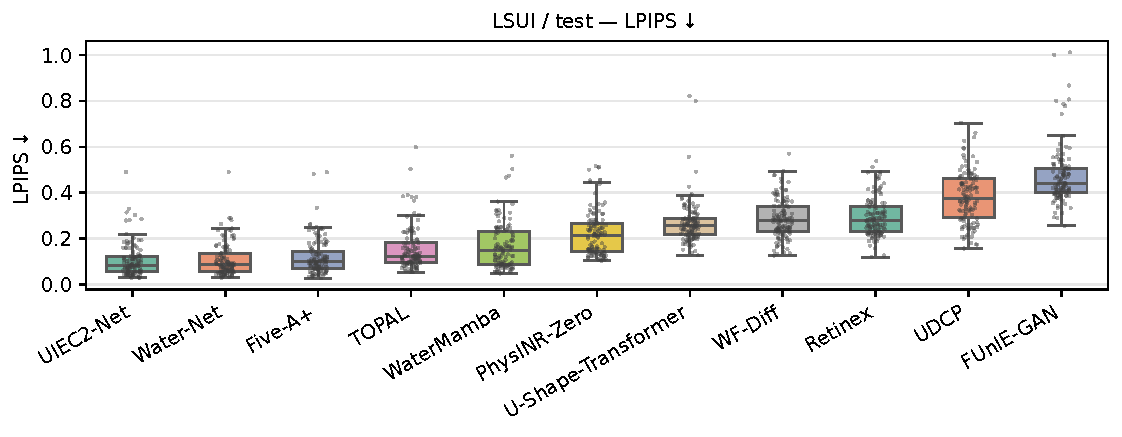
\includegraphics[width=0.48\textwidth]{box_LSUI_lpips_alex.pdf}
\hfill
\caption*{\textbf{S2} LSUI score distributions for all eleven methods (PSNR, SSIM, MS-SSIM, LPIPS-AlexNet).}
\end{figure}

\begin{figure}[htbp]
\centering
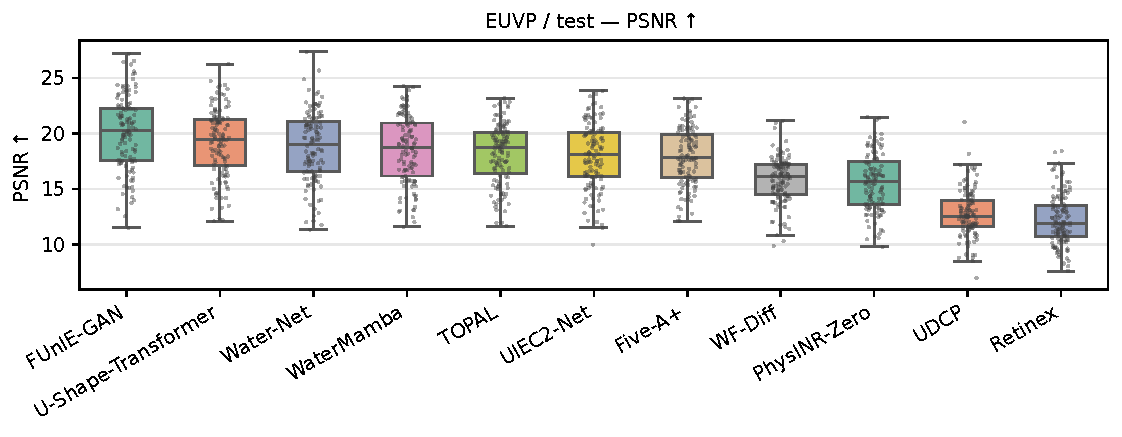
\includegraphics[width=0.48\textwidth]{box_EUVP_psnr.pdf}
\hfill
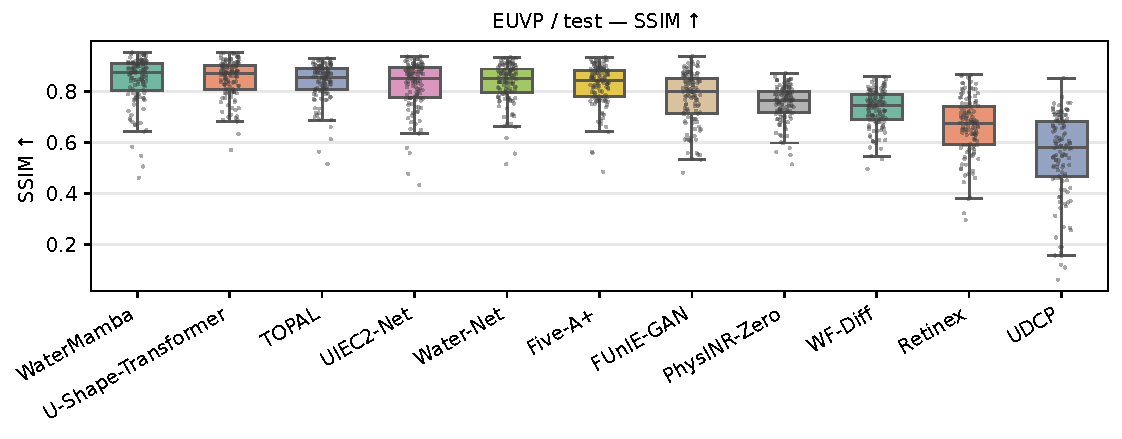
\includegraphics[width=0.48\textwidth]{box_EUVP_ssim.pdf}
\hfill
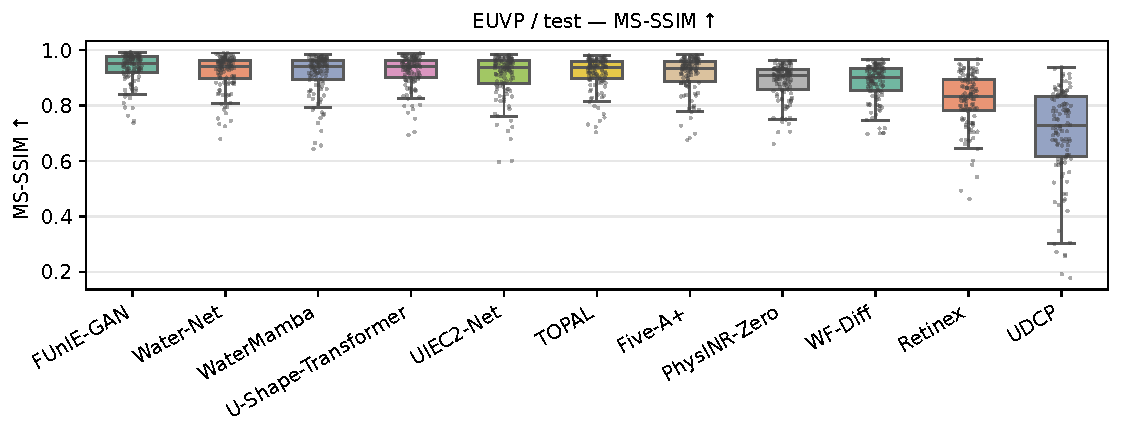
\includegraphics[width=0.48\textwidth]{box_EUVP_ms_ssim.pdf}
\hfill
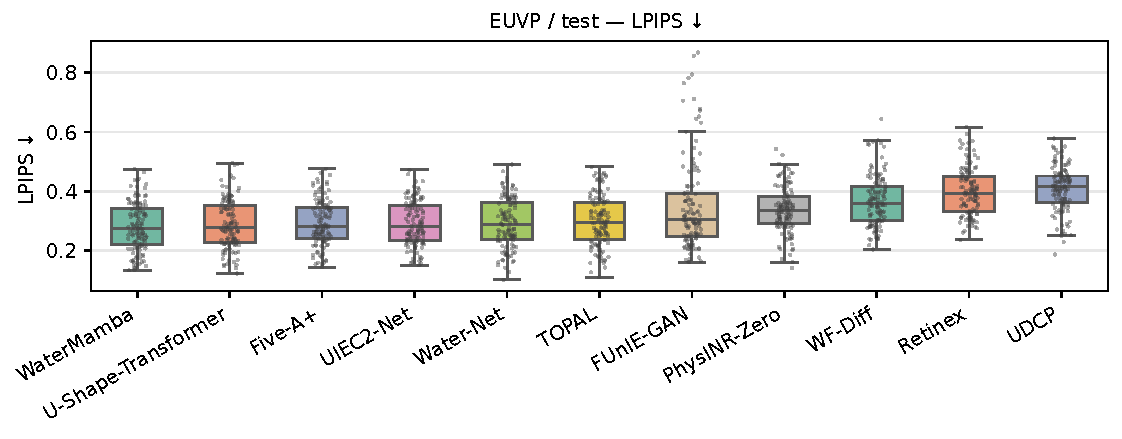
\includegraphics[width=0.48\textwidth]{box_EUVP_lpips_alex.pdf}
\hfill
\caption*{\textbf{S3} EUVP score distributions for all eleven methods (PSNR, SSIM, MS-SSIM, LPIPS-AlexNet).}
\end{figure}

\begin{figure}[htbp]
\centering
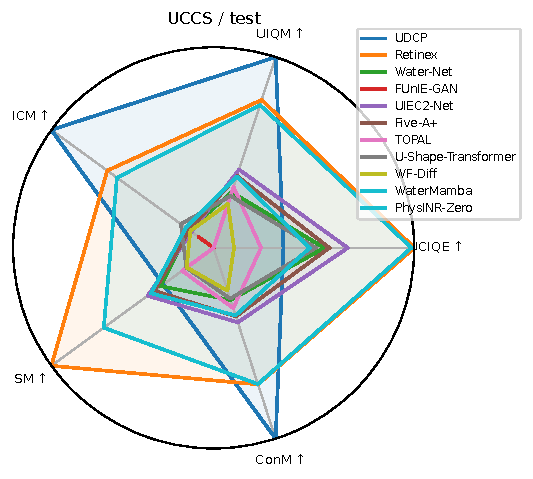
\includegraphics[width=0.48\textwidth]{radar_UCCS.pdf}
\hfill
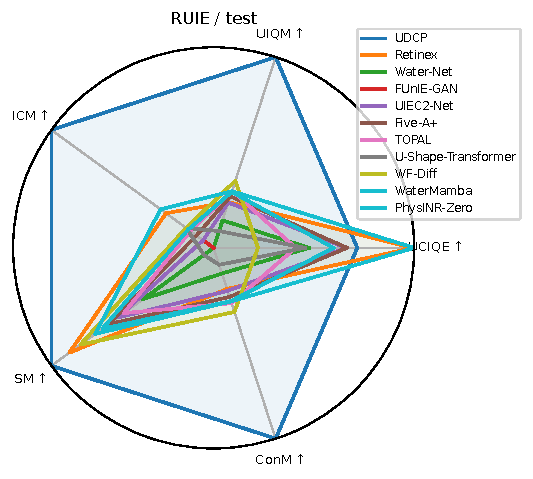
\includegraphics[width=0.48\textwidth]{radar_RUIE.pdf}
\hfill
\caption*{\textbf{S4} No-reference profiles (UCIQE, UIQM, UICM, UISM, UIConM) on UCCS and RUIE.}
\end{figure}

\end{document}